\let\negmpace\undefined
\let\negthickspace\undefined
\documentclass[journal]{IEEEtran}
\usepackage[a5paper, margin=10mm, onecolumn]{geometry}
%\usepackage{lmodern} % Ensure lmodern is loaded for pdflatex
% Include tfrupee package
\setlength{\headheight}{1cm} % Set the height of the header box
\setlength{\headsep}{0mm}     % Set the distance between the header box and the top of the text
\usepackage{xparse}
\usepackage{gvv-book}
\usepackage{gvv}
\usepackage{cite}

\usepackage{amsmath,amssymb,amsfonts,amsthm}
\usepackage{algorithmic}
\usepackage{graphicx}
\usepackage{textcomp}
\usepackage{xcolor}
\usepackage{txfonts}
\usepackage{listings}
\usepackage{enumitem}
\usepackage{mathtools}
\usepackage{gensymb}
\usepackage{comment}
\usepackage[breaklinks=true]{hyperref}
\usepackage{tkz-euclide} 
\usepackage{listings}
% \usepackage{gvv}                                        
\def\inputGnumericTable{}                                 
\usepackage[latin1]{inputenc}                                
\usepackage{color}                                            
\usepackage{array}                                            
\usepackage{longtable}                                       
\usepackage{calc}                                             
\usepackage{multirow}                                         
\usepackage{hhline}                                           
\usepackage{ifthen}                                           
\usepackage{lscape}
\renewcommand{\thefigure}{\theenumi}
\renewcommand{\thetable}{\theenumi}
\setlength{\intextsep}{10pt} % Space between text and floats
\numberwithin{equation}{enumi}
\numberwithin{figure}{enumi}
\renewcommand{\thetable}{\theenumi}
\begin{document}
\bibliographystyle{IEEEtran}
\title{9.4.4}
\author{EE24BTECH11033 - KOLLURU SURAJ}
% \maketitle
% \newpage
% \bigskip
{\let\newpage\relax\maketitle}
\textbf{Question:} 
$\sec^2 x \tan y \, dx + \sec^2 y \tan x \, dy = 0$
\\\\
\solution\\
Divide the given equation with $\tan x \tan y$
\begin{align}
    \frac{\sec^2 x \, dx}{\tan x} + \frac{\sec^2 y \, dy}{\tan y} = 0\\
    \frac{dy}{dx}=-\frac{sin2y}{sin2x}\label{1}
\end{align}
Substitute $\tan x$ as u and $\tan y$ as v
\begin{align}
    \frac{du}{u} + \frac{dv}{v} = 0
\end{align}
Integrate
\begin{align}
\int  \frac{du}{u} + \int \frac{dv}{v} = \int 0\\
    \ln u + \ln v = a\\
    \ln uv = a\\
    \tan x \tan y = e^a
\end{align}
 $e^a$ can be written as another constant $c$
 \begin{align}
      \tan x \tan y = c
 \end{align}
Here no initial condition is given so let us take $X_{0}=\pi/4,Y_{0}=\pi/4$ which gives $c=1$
\begin{align}
    \tan x \tan y = 1\\
    \tan y = \cot x\\
    y = \tan^{-1}(\cot x)\\
    y= \frac{\pi}{2}- x
\end{align}
Now let us  this computationally from the definition of $\frac{dy}{dx}$ 
\begin{align}
    Y_{n+1}=Y_n+\frac{dy}{dx}\cdot h
\end{align}
From the differential equation \ref{1}
\begin{align}
    \frac{dy}{dx}=-\frac{\sin 2y}{\sin 2x}\\
    y_{n+1}=y_n-\frac{\sin 2y_n}{\sin 2x_n}\cdot h
\end{align}
BY taking $x_0$=0 and $y_0$=1 and h=0.01  by iterating through the loop a 100 times and finding $y_2,y_3,y_4,\cdots$ and plotting the graph. we can verify the function we got by solving the differential equation mathematically

\begin{figure}[!ht]
    \centering
    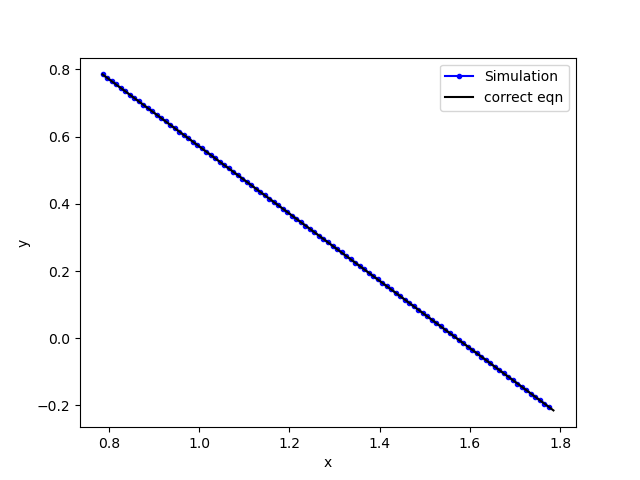
\includegraphics[width=\columnwidth]{figs/Figure_1.png}
    \caption{}
\end{figure}


\end{document}
